\section{Evaluation}
% Met een subsectie voor elke deelvraag.
% In hoeverre is je vraag beantwoord?
% Een mooie graphic/visualisatie is hier heel gewenst.
% Hou het kort maar krachtig.

\subsection{RQ1}
For answering what pooling technique pairs best with each embedding technique, a logistic regression has been performed to test which pooling technique results in the highest accuracy.
Before that, however, a regularization type needs to be specified. 

\begin{figure}[h]
    \centering
    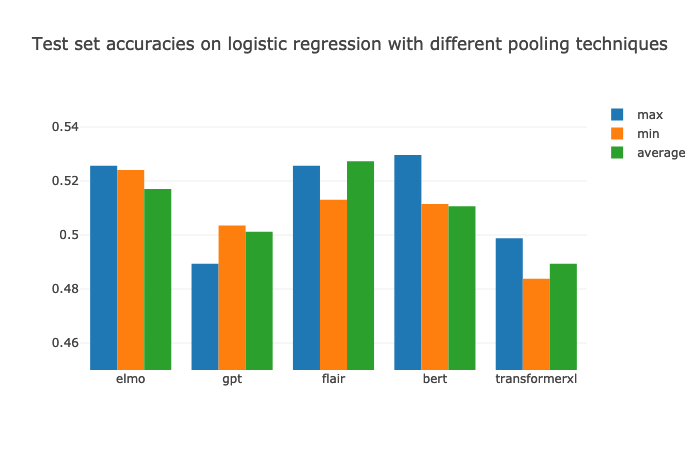
\includegraphics[scale=0.5]{poolingaccuracy}
    \caption{Comparing different pooling strategies.}
\end{figure}

\subsection{RQ2}
To answer the question which sequence length is optimal for neural classification, data with variable maximum lengths have been fed into bidirection LSTMs and convolutional neural networks.
For these maximum lengths, the lengths between two standard deviations from the median of the total word lengths per statement have been used, as is illustrated in figure 4. 
In this figure, the lowest maximum length, the median and the highest length are shown.

\begin{figure}
    \centering
    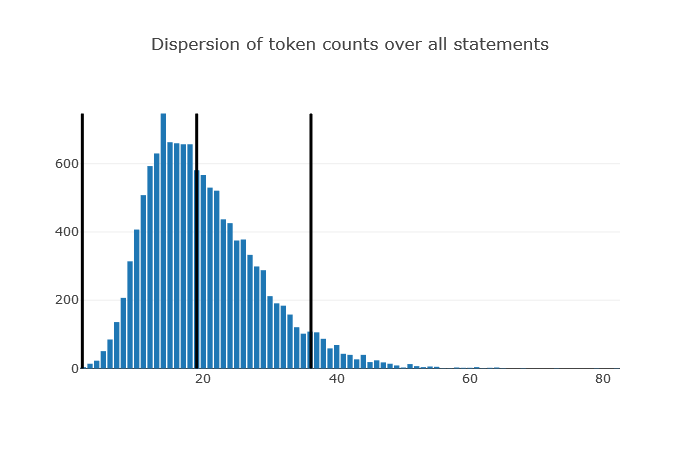
\includegraphics[scale=0.5]{wordlength}
    \caption{Total token counts per statement on the Liar dataset.}
\end{figure}

\begin{figure}[h]
    \centering
    \begin{subfigure}[b]{1\textwidth}
       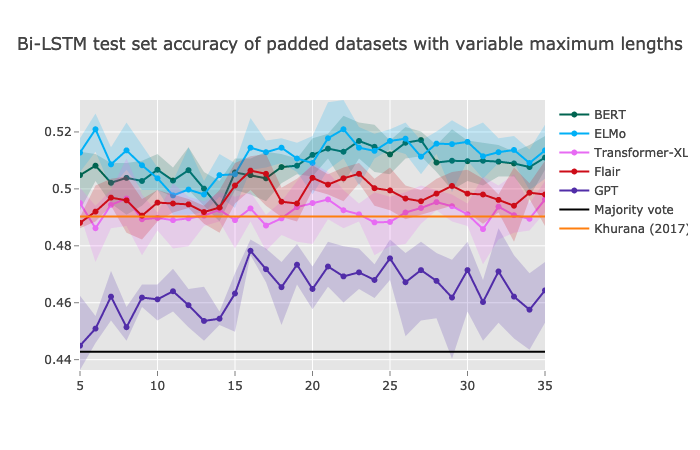
\includegraphics[width=1\linewidth]{bilstmaccuracies}
       \caption{Bidirectional LSTM accuracies.}
    \end{subfigure}
    
    \begin{subfigure}[b]{1\textwidth}
       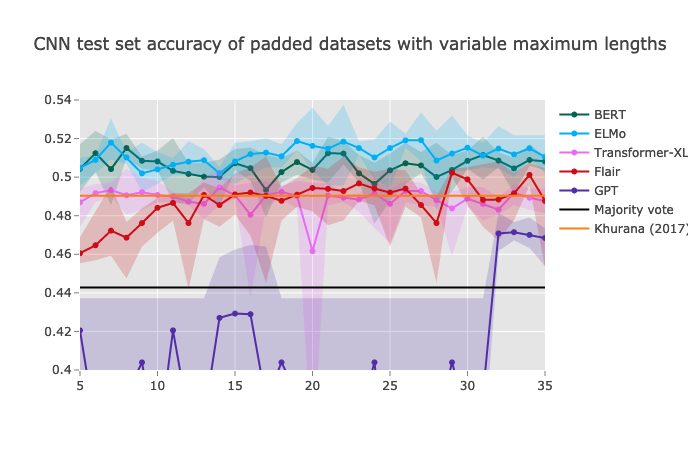
\includegraphics[width=1\linewidth]{cnnaccuracies}
       \caption{Convolutional neural network accuracies.}
    \end{subfigure}
    
    \caption{Test set accuracies with variable maximum lengths over neural network architectures.}
\end{figure}

In figure 5\todo{Check if this number is still correct}, the accuracies with different amounts of padding can be seen, compared to our 3 baselines.

\subsection{RQ3}
\textbf{How well do neural network classification architectures classify fake news compared to non-neural classification algorithms?}\\
The answer of this question will be given by comparing two linear classifiers with two neural classifiers. 

\begin{figure}[h]
    \centering
    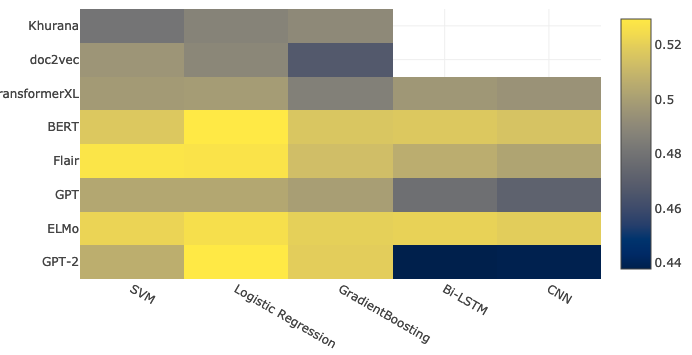
\includegraphics[scale=0.5]{linearvsneural}
    \caption{Comparing linear classifiers with neural classifiers.}
\end{figure}

\pagebreak